\chapter{Analyse de domaine}
\begin{preamble}
Dans ce chapitre nous analysons une variété de couches de traitement de données dans le domaine du vieillissement à domicile pour identifier les concepts clés et les opérations spécifiques pour le traitement de la sensibilité au contexte. Reposant sur cette analyse, nous proposons un langage sensible au contexte, dédié, et son architecture logicielle, qui permet de mettre en synergie les intervenants d'une maison sensible au contexte, en leur fournissant une approche unifiée pour concevoir et développer des services.
\end{preamble}
\chpsummary{Contributions}
{
{\em Domain analysis} We provide an analysis of context-aware processing layers in the domain of aging in place. From this analysis, we identify key concepts and operations specific to context-aware processing.;
{\em Domain-specific language} We introduce a language, specific to developing context-aware services, providing high-level abstractions and notations. 
Underlying this language is a data-centric and data-driven paradigm that allows services from a range of stakeholders to uniformly process heterogeneous sources of sensed data.;
%\myparagraph{Compiler} We have implemented a compiler for our DSL that maps high-level rules into low-level requests, crunched by an event-processing engine.
{\em Validation} We applied our approach to re-implement 55 services, ranging over all the stakeholders of an assisted living platform dedicated to aging in place. The resulting services are expressed at a high level and are effective in performing the tasks of the stakeholders.
}


La notion de {\em contexte} est fondamentales dans les champ de l'informatique ubiquitaire et englobe de beaucoup de dimensions, 


The notion of {\em context} is fundamental to the field of pervasive computing and encompasses a range of dimensions, including the physical world, an individual, their activities, and their technologies~\cite{bauer2012comparison}. 
% This wide range of dimensions is reflected in the host of application areas that leverages context awareness, spanning infrastructures ({\em e.g.,} railways), premises ({\em e.g.,} buildings), and health ({\em e.g.,} physiological status). 
A major focus of the research on context awareness has been the {\em home} ({\em e.g.,}~\cite{cook2013casas,feminella2014piloteur}). This scope involves many context dimensions, including physical interactions with the environment ({\em i.e.,} sensors), digital interactions with the user environment ({\em e.g.,} email, calendar), status of the many components of the pervasive computing infrastructure (hardware, software, and network), application-specific concerns ({\em e.g.,} activity detection). When it comes to context-aware homes for the general population, a recurring challenge is to identify what services users would need~\cite{brush2011home}, and more generally, to develop methods to gather and analyze these needs~\cite{coutaz2010disqo}.

% explores usage scenarios that do not necessarily apply to the pressing needs of a given population and involves studies that are mostly conducted in an experimental setting. Towards validating context-aware home, a realistic setting is required, involving daily scenarios that revolve around context awareness.

% a major societal challenge where pervasive computing can play a key role

However, when focusing on older adults, this population is ready to benefit from context-aware homes to support aging in place. A pervasive computing environment has the potential to deliver assistive services 24/7 and address the needs of older adults, whose nature can be of utmost importance to ensure independent living ({\em e.g.,} ~\cite{rashidi2013survey}). These services mainly consist of 1) detecting and reminding daily activities ({\em e.g.,} meal preparation, self-care, going to bed) to maintain the user's functional status~\cite{caroux2014verification} and 2) monitoring potentially hazardous situations ({\em e.g.,} cooker, entrance door) to make the user safe~\cite{rashidi2013survey}. Because it crosscuts various fields, a context-aware home dedicated aging in place involves a variety of stakeholders to design and develop assistive services, as well as to deploy and maintain the underlying infrastructure. Stakeholders include older users, caregivers, aging experts, health professionals, application developers, and maintenance technicians. This considerable diversity of stakeholders raises correspondingly diverse context dimensions. Typically, each stakeholder develops their own, silo-based approach to extracting their specific context information from sensed data.

We analyzed existing data processing layers of multiple stakeholders, extracted from an assisted living platform, deployed in 129 single-occupant homes of older adults, aged 82 years old on average~\cite{consel2017homeassist}. This case study thus consists of a range of services, whose usefulness has been validated in practice on a daily basis. Our analysis identifies commonalities and variabilities of these layers, revealing key concepts and operations specific to context-aware processing. 

\subsection*{Our Approach}
Based on this analysis, we propose a context-aware, domain-specific language and its software architecture, which provide a conceptual framework and a tool to unify the design and the development of home services. To unify heterogeneous sources of sensed data, ranging from hardware devices to software components, our approach promotes a processing paradigm, which is data centric and data driven. Specifically, our approach is {\em data centric} to provide a canonical view of sensed data to a range of services, spanning maintenance services consuming low-level device status, to caregiving-specific services using high-level activity measures. Our approach is {\em data driven} in that services are defined in terms of rules processing events and states.

To unify the way services are developed, our approach introduces abstractions and notations that are specific to context-aware processing. The resulting {\em domain-specific language} (DSL) covers the needs of the stakeholders and provides an abstraction layer over underlying, well-established concepts and technologies, such as Allen's algebra to express sequences of interactions~\cite{Allen} and complex-event-processing engines to efficiently process the rules generated from DSL services ({\em e.g.,}~\cite{Cugola:2012:PFI:2187671.2187677}). Furthermore, we envision that our language can serve as a high-level stepping stone to introduce end-user programming languages for stakeholders with no computer-programming background.

To validate our approach, we have re-implemented 55 services ranging over all the stakeholders of the assisted living platform under study. These new services were deployed and successfully tested for their effectiveness in performing the specific tasks of the stakeholders: detection of daily activities, detection of user risks, sensor failure, {\em etc.}

\subsection*{Contributions}
To summarize, this paper makes the following contributions.

\myparagraph {Domain analysis} We provide an analysis of context-aware processing layers in the domain of aging in place. From this analysis, we identify key concepts and operations specific to context-aware processing.

\myparagraph {Domain-specific language} We introduce a language, specific to developing context-aware services, providing high-level abstractions and notations. 
Underlying this language is a data-centric and data-driven paradigm that allows services from a range of stakeholders to uniformly process heterogeneous sources of sensed data.

\myparagraph{Compiler} We have implemented a compiler for our DSL that maps high-level rules into low-level requests, crunched by an event-processing engine.

\myparagraph {Validation} We applied our approach to re-implement 55 services, ranging over all the stakeholders of an assisted living platform dedicated to aging in place. The resulting services are expressed at a high level and are effective in performing the tasks of the stakeholders.





\section{Domain analysis}
Context-aware homes for aging in place are still in their infancy and the path to adoption is being actively researched~\cite{kaye2017making}. The literature include few articles reporting on the deployment of assisted living platforms in the wild ({\em e.g.,} \cite{kaye2011intelligent}). Fortunately, we have been able to leverage the {\em HomeAssist} project to conduct a domain analysis of context-aware homes for aging in place. 

\subsection{HomeAssist: A Context-Aware Home for Aging in Place}
HomeAssist is an assisted living platform that provides a catalog of assisted applications, supporting daily activities, safety and social participation~\cite{consel2017homeassist}. HomeAssist has been deployed in 129 single-occupant homes of community-dwelling older adults, 82 years old on average. The duration of this field study is 12 months.

HomeAssist is a perfect case study on which to build a unifying approach to developing context-aware home services dedicated to aging in place. It matches all the requirements to pursue our goal: 1) it is deployed in the wild in real homes; 2) it supports aging in place for frail users with pressing needs; 3) the field study is long enough that maintenance and evolution problems must be properly handled; 4) it is deployed at a large enough scale that administering context-aware homes need to be supported by services; 5) existing services reflect a range of needs expressed by stakeholders, spanning older users, caregivers, occupational therapists, psychologists, human factors experts, installation and maintenance technicians, and computer scientists.

Let us further describe this platform to delimit the scope of the issues raised by the context-aware services. HomeAssist consists of a client-server architecture, where the server runs as many virtual machines as they are context-aware homes. Each virtual machine executes the assistive services selected by the user and their caregiver. These assistive services are fed with sensing data sent via Internet by a gateway, deployed in the context-aware home. This gateway gathers information from the sensors placed at strategic locations in the older adult's home to monitor their daily activities (see Caroux {\em et al.} for more details~\cite{caroux2014verification}). As well, the gateway channels actions from the services to the home's actuators. In the HomeAssist field study, a typical home consists of 4 contact sensors (entrance door, drawers, cabinets, {\em etc.}), 6 motion detectors (entrance area, kitchen, bathroom, {\em etc.}), and 2 smart plugs, which measure the electricity consumption and turn on/off a connected appliance (microwave, light path, coffeemaker, {\em etc.}). The number and type of devices can vary depending on the configuration of the home and the activities to be monitored. Finally, the home is equipped with a stationary tablet, placed at a central location in the home and always connected to a power outlet. This tablet is dedicated to interacting with the user via notifications emitted by assistive applications, which need to alert the user of a given situation ({\em e.g.} unattended entrance door left open)~\cite{consel2015unifying}.

% Let us now illustrate the diversity of issues addressed by HomeAssist with a set of existing scenarios dedicated to support aging in place.

\begin{figure*}[t]
\begin{tabular}{| l | l | l | p{7cm} |} \hline
{\bf Stakeholder} & {\bf Domain} & {\bf Name} & {\bf Description} \\ \hline \hline
Older adult& Safety & Door Alert & Entrance door \uline{is open} and  \uline{is unattended} \dotuline{for 5 minutes} \\ \hline
Caregiver & \begin{tabular}{ll} Daily \\ Activities \end{tabular} 
       & \begin{tabular}{ll} Reheating \\ A Frozen Meal\end{tabular} 
          & Freezer \dashuline{gets used} and stove \dashuline{gets turned on} \dotuline{within 10 minutes} or Freezer \dashuline{gets used} during stove \uline{is on},
during \uline{lunch time} (or dinner time) \\ \hline
\begin{tabular}{ll} Home \\Technician \end{tabular}
               & Maintenance & \begin{tabular}{ll} Presence \\ Dependency\end{tabular} 
                  & Whenever the cupboard \dashuline{gets opened} in the kitchen, a presence in the kitchen \uline{is true} \\ \hline
\begin{tabular}{ll} Home \\Technician \end{tabular}
   & Maintenance 
        & \begin{tabular}{ll} Communication \\ Failure \end{tabular} 
             & A sensor \uline{fails to communicate} \dotuline{for 24 hours} and its status does not \dashuline{get updated} \\ \hline
\end{tabular}
\caption{Example scenarios for assistive services}
\label{scenario-fig}
\end{figure*}


%**********************************************
\subsection{Scenarios To Support Aging In Place}\label{domain:scenario}
%\cc{Remplacer les couleurs par des soulignes pleins et pointilles (par ex) pour ne pas dependre de la couleur.}

We now present four scenarios that illustrate the spectrum of stakeholders and concerns involved in supporting aging in place with a context-aware home (see Figure~\ref{scenario-fig}). The first scenario addresses the safety concern of the older adult. It consists of monitoring the entrance door to ensure that it is not left open for too long without being attended. The second scenario relates to a caregiver's need to monitor a user's daily activities, and in particular, their eating routines. The last two scenarios address the home technician's concerns to keep the context-aware home in an operational state. The first maintenance scenario detects inconsistent values produced, or values omitted, by the motion detector of the kitchen. This situation is discovered by cross-checking the motion detector information  with that of the contact sensor of the cupboard (or any other sensor located in that room). The second maintenance scenario detects whether a sensor fails to communicate; this situation occurs when the sensor has a drained battery or is malfunctioning.

These scenarios offer a glimpse at the kind of context-aware services needed to support aging in place. Some services, such as ``Door Alert'', can fit most older users. Other services may target daily activities that require a level of personalization for an effective monitoring. This is illustrated by the meal preparation activity and the ``Reheating a Frozen Meal'' scenario. 

Similarly, for maintenance scenarios, ``Communication Failure'' applies to any context-aware home, whereas ``Presence Dependency'' requires to instantiate the consistency rules with respect to the locations of sensors.

% We are now ready to further examine home services for aging in place, as illustrated in Figure~\ref{scenario-fig}, to extract their commonalities and variabilities, as a basis to raise the level of abstraction to express such services.

% We defined scenarios from stakeholders requirements that daily use a computing assistive platform.
% \subsubsection*{Home safety: Door alert}
% Entrance door \colorbox{teal!15}{is unattended} \colorbox{blue!5}{for 5 minutes}
% \subsubsection*{Infrastructure status: Presence dependency}
% When the cupboard \colorbox{checked!10}{gets opened} in the kitchen, a presence in the kitchen \colorbox{teal!15}{is true} 
% \subsubsection*{Activity monitoring: Lunch Warmup}
% Freezer \colorbox{checked!10}{gets used} and stove \colorbox{checked!10}{gets turned on} \colorbox{blue!5}{within 10 minutes} or Freezer \colorbox{checked!10}{gets used} during stove \colorbox{checked!10}{is on} \\
% during \colorbox{teal!15}{lunch time}
% \subsubsection*{Sensor monitoring: Commfailure alert}
% A sensor \colorbox{teal!15}{is in commfailure} \colorbox{blue!5}{for 24 hours} and its status does not \colorbox{checked!10}{get updated}
% Caption:
% \begin{itemize}
% \itshapeem\colorbox{teal!15}{State}, \colorbox{checked!10}{event}, \colorbox{blue!5}{duration}
% \end{itemize}


\subsection{Commonality and Variability Analysis}
To conduct our domain analysis, we have examined a range of services offered by HomeAssist to identify their commonalities and variabilities. These services were developed in Java using a tool-based design methodology~\cite{bertran2014diasuite,cassou2012toward}.

We now present the outcomes of this analysis that take the form of high-level, domain-specific concepts. These concepts will pave the way to our domain-specific approach presented in the next section.

\myparagraph{Commonalities} All services refer to a notion of {\em environment} from which to perform measures. These measures encompass interactions in both a physical environment ({\em e.g.,} a motion detected) and  a digital one ({\em e.g.,} an event reminder issued by a calendar). Additionally, we identified two complementary concepts related to an environment: events and states. On the one hand, an {\em event} defines an environment measure that changes ({\em e.g.,} door {\em gets} closed/open) -- events are underlined with a dashed line in the scenarios of Figure~\ref{scenario-fig}. On the other hand, a {\em state} makes an event persistent across time ({\em e.g.,} door {\em is} open) -- states are underlined with a solid line in Figure~\ref{scenario-fig}. Once these unitary concepts were identified, we found specific ways in which they can be combined, revealing {\em composition} commonalities. Specifically, the combination of environment measures can define an {\em order} in which interactions must occur and their {\em duration} -- these constraints are underlined with a dotted line in Figure~\ref{scenario-fig}.

Let us further study these commonalities by examining their range of variability.

\myparagraph{Variabilities} Environmental measures may be realized by a variety of entities, hardware ({\em e.g.,} sensor), software ({\em e.g.,} calendar), local ({\em e.g.,} door), remote ({\em e.g.,} new email messages), {\em etc.} The abstraction level of the environmental measures varies widely. For example, an event may be produced by a sensor, as soon as a motion is detected in a room. Alternatively, a sensor may detect the state of a room being occupied, excluding room-to-room transfers.

Regarding composition, several order constraints were observed between interactions, including an interaction {\em preceding} another one, an interaction occurring {\em during} another one, and an interaction {\em overlapping} another one. Not all of these constrains are applicable to any kind of interactions ({\em i.e.,} event and state). For example, only two states may overlap, whereas two events cannot. Indeed, in practical scenarios, events are viewed as occurring sequentially, not simultaneously.



\section{A DSL For Context-Aware Services}\label{sec:dsl}

We now present the main stages of our domain-specific approach to developing context-aware services dedicated to aging in place. This approach is depicted in Figure~\ref{fig:functionalarchi}.

\begin{figure}[h]
\centering
  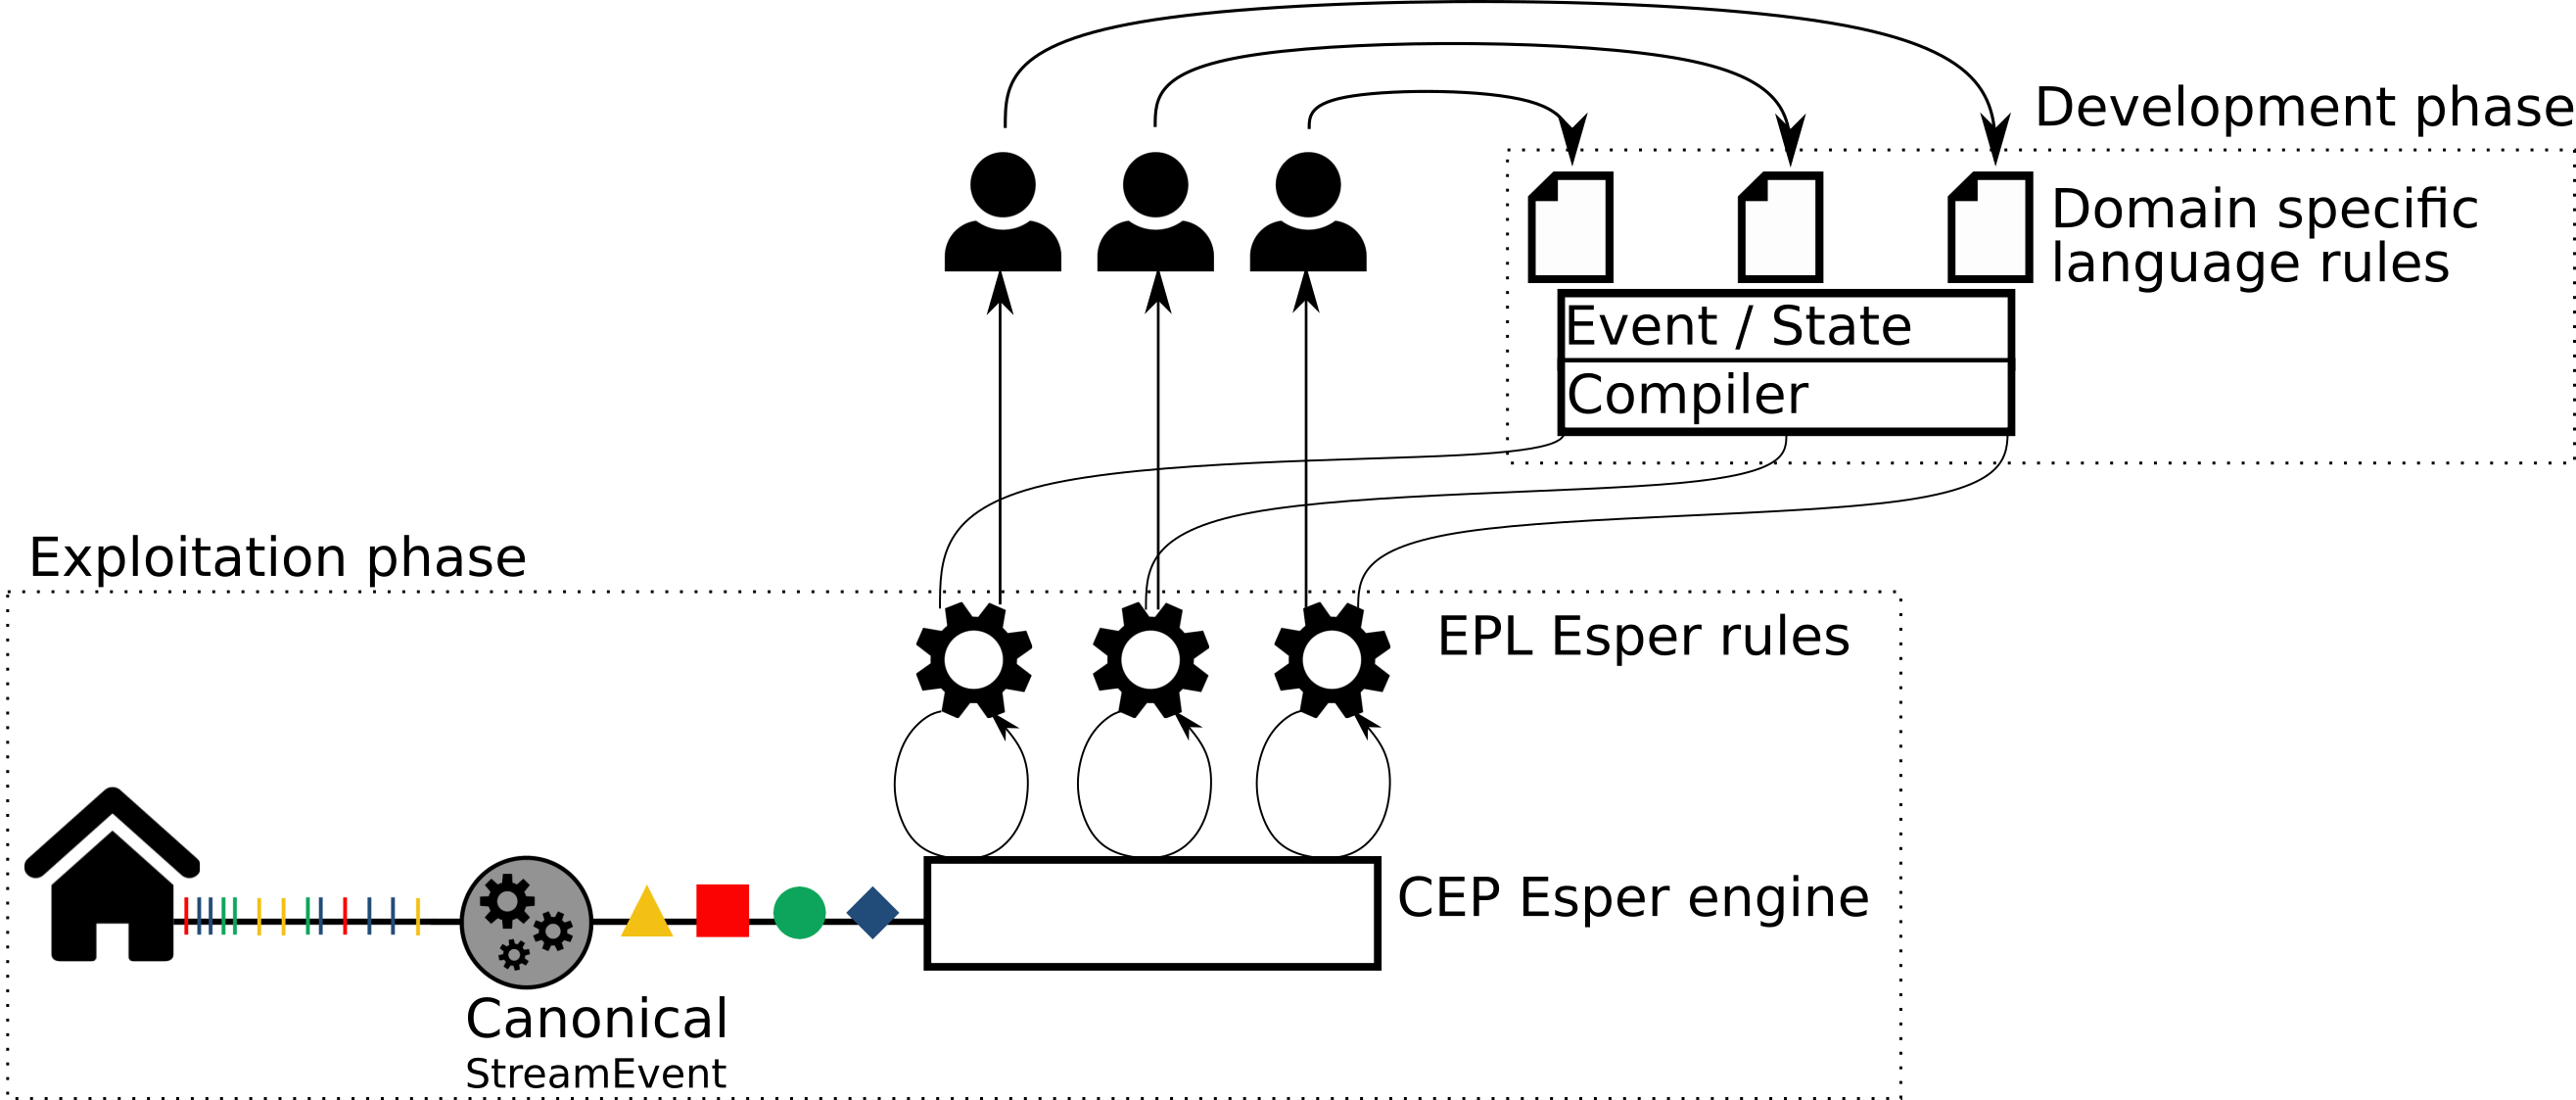
\includegraphics[scale=0.13]{gfx/approach}
\caption{Overall view of our domain-specific approach}
\label{fig:functionalarchi}
\end{figure}


\subsubsection{Service definition}
The first step is initiated with the stakeholders that express scenarios of services, as illustrated earlier. These scenarios are directly written in our domain-specific language (see next section) by the stakeholders, if they have the proper background, or by a service developer. 

\subsubsection{Service compilation}
The high-level service is compiled into low-level rules written in an event processing language. These rules make explicit the domain-specific concepts, such as states that are compiled into a combination of events and related operations.

\subsubsection{Service execution}
When deployed, the rules are added to a Complex Event-Processing (CEP) engine.  Our rule execution engine is based on Esper, an open source CEP developed by EsperTech.\footnote{http://www.espertech.com/esper/}  It offers Java and C\# interfaces to develop event-based programs.  We chose Esper because it is a popular CEP engine, used both in industry and research.  Esper contains a declarative domain-specific language for CEP, called EPL (for Event Processing Language).  EPL allows to describe patterns of events to be recognized in an online stream of events, using operators for ordering events, time constraints, alternatives, {\em etc.} Esper does not offer a concept of state; it only handles events and requires extra machinery to manage a state.  In our implementation, we run the Esper engine with respect to EPL rules, compiled from our DSL rules, and a stream of events from the context-aware home, formatted in a canonical form.

\subsubsection*{Canonical form}
The canonical form of sensed data produced by context-aware homes allows to process them uniformly, disregarding their original heterogeneous formats.  In our implementation, the canonical form of data, called {\em StreamEvent}, is introduced as an abstraction layer above the flow of sensed data events. In this representation, each event consists in a 4-tuple consisting of the kind of event, its location, its value, and the timestamp of its occurrence.



In this section, we introduce our DSL for developing context-aware services. This DSL is dedicated to describing contexts in terms of states and events, and operators to combine them. Figure~\ref{fig:operators}  presents the syntax of our DSL, as well as its informal semantics. Each construct of the language is presented on the left-hand side; its corresponding graphical representation is displayed on the right-hand side. This graphical representation visualizes events and states, and how operators combine them. A state is represented as a rectangle-shaped signal, visualizing the starting and ending points of the occurrence of an event. An event is represented as a spike signal, with merged starting and ending points. Underneath each DSL construct is its translation into a core DSL, which can be viewed as an abstract syntax.

%% example greater less
%variant : precedes less, precedes greater
\begin{figure*}[ht]
\begin{center}
  \begin{tikzpicture}[node distance=\dx and \dy,
    >=latex,shorten >=2pt,shorten <=2pt,auto,
    semithick,initial distance=1cm,
    every initial by arrow/.style={*->} ]
    \draw[gray!50,line width=0.1mm,dashed] (-1.5,.5) -- (-1.5,-1.2);
    \draw[gray!50,line width=0.1mm,dashed] (1.5,.5) -- (1.5,-1.2);  
    \draw[gray!50,line width=0.1mm,dashed] (-.5,.2) -- (-.5,-1.);
    \draw[gray!50,line width=0.1mm,dashed] (.5,.2) -- (.5,-1.);  
    \draw[] (-1.5,.) 
    node[xshift=-2.8 cm,yshift=.125cm] {\scriptsize Event:} 
    node[xshift=-1.5 cm,yshift=.25cm] {\scriptsize {\tt p {\em becomes} v}} 
    node[xshift=-1.5 cm,yshift=. cm] {\scriptsize $p\Rightarrow v$} 
    node[xshift=-.2 cm,yshift=0 cm] {\scriptsize {\tt e}} --(-.5,.)--(-.5,.4) -- (-.5,.) -- (1.5,.);
    % \draw[] (-1.5,.-.6) 
    % node[xshift=-2.8 cm,yshift=.125cm] {\scriptsize Event:} 
    % node[xshift=-1.5 cm,yshift=.25cm] {\scriptsize {\tt p {\em becomes} v'}} 
    % node[xshift=-1.5 cm,yshift=. cm] {\scriptsize $p\Rightarrow v$} 
    % node[xshift=-.2 cm,yshift=0 cm] {\scriptsize {\tt e}} --(.5,-.6)--(.5,-.2) -- (.5,-.6) -- (1.5,-.6);
    \draw[] (-1.5,-.6) 
    node[xshift=-.12 cm,yshift=.25cm] {\scriptsize ${\tt v}$} 
    node[xshift=-.1 cm,yshift=. cm] {\scriptsize ${\tt v'}$} 
    node[xshift=-.25 cm,yshift=.125 cm] {\scriptsize {\tt p}} -- (-.5,-.6) -- (-.5,-.2) -- (.5,-.2) -- (.5,-.6) -- (1.5,-.6);
    \draw[] (-1.5,-1.2) 
    node[xshift=-2.8 cm,yshift=.125cm] {\scriptsize State:} 
    node[xshift=-1.5 cm,yshift=.25cm] {\scriptsize {\tt p {\em is} v}} 
    node[xshift=-1.5 cm,yshift=. cm] {\scriptsize $p=v$} 
    node[xshift=-.2 cm,yshift=0 cm] {\scriptsize {\tt s}} -- (-.5,-1.2) -- (-.5,-.8) -- (.5,-.8) -- (.5,-1.2) -- (1.5,-1.2);
    
  \end{tikzpicture}
\end{center}
  \begin{multicols}{2}
    \begin{tikzpicture}[node distance=\dx and \dy,
      >=latex,shorten >=2pt,shorten <=2pt,auto,
      semithick,initial distance=1cm,
      every initial by arrow/.style={*->} ]   
      \draw[gray!50,line width=0.1mm,dashed] (-1.5,.5) -- (-1.5,-1.2);
      \draw[gray!50,line width=0.1mm,dashed] (1.5,.5) -- (1.5,-1.2);  
      %%%%%%%%%%%%%%%%%%%%%%%%%%%%%%%%%%%%%%%%%%%%%%%%%%%%%%%%%%%%%%%%%%%%%%%
      \draw[gray!50,line width=0.1mm,dashed] (.5,.) -- (.5,-1.2);   
      \draw[] (-1.5,.) 
      node[xshift=-.25 cm,yshift=.125cm] {\scriptsize {\tt e$_1$}}  --(-.5,.)--(-.5,.4) -- (-.5,.) -- (1.5,.);
      \draw[] (-1.5,-.6) 
      node[xshift=-.25 cm,yshift=.125cm] {\scriptsize {\tt e$_2$}} -- (.5,-.6) -- (.5,-.2) -- (.5,-.6) -- (1.5,-.6);
      \draw[] (-1.5,-1.2) 
      node[xshift=-3.4 cm,yshift=.5cm] {\scriptsize Every time {\tt e$_1$} {\em immediately} precedes {\tt e$_2$}}
      node[xshift=-3. cm,yshift=.25cm] {\scriptsize {\tt e$_1$ {\bf precedes} e$_2$ $\Leftrightarrow$ $Precedes(e_1,e_2)$}}
      node[xshift=-4.5 cm,yshift=-.45cm] {\scriptsize Variants:}
      node[xshift=-0.55 cm,yshift=-.4cm] {\scriptsize {\tt e$_1$ {\bf precedes within} t e$_2$ $\Leftrightarrow$ $Precedes\_less(t)(e_1,e_2)$}}
      node[xshift=-0.525 cm,yshift=-.65cm] {\scriptsize {\tt e$_1$ {\bf precedes by} t e$_2$ $\Leftrightarrow$ $Precedes\_greater(t)(e_1,e_2)$}} -- (.5,-1.2) -- (.5,-.8) -- (.5,-1.2) -- (1.5,-1.2);
      %%%%%%%%%%%%%%%%%%%%%%%%%%%%%%%%%%%%%%%%%%%%%%%%%%%%%%%%% 
      \draw[gray!50,line width=0.1mm,dashed] (-1.5,-2.) -- (-1.5,-3.7);
      \draw[gray!50,line width=0.1mm,dashed] (1.5,-2.) -- (1.5,-3.7);  
      \draw[gray!50,line width=0.1mm,dashed] (-.5,-2.5) -- (-.5,-3.7);   
      \draw[gray!50,line width=0.1mm,dashed] (.,-2.5) -- (.,-3.7);  
      \draw[gray!50,line width=0.1mm,dashed] (.5,-2.5) -- (.5,-3.7);
      \draw[] (-1.5,-2.5) 
      node[xshift=-.25 cm,yshift=.125cm] {\scriptsize {\tt e}} --(-.5,-2.5)--(-.5,-2.1)--(-.5,-2.5)--(.,-2.5)--(.,-2.1)--(.,-2.5)--(.5,-2.5)--(.5,-2.1)--(.5,-2.5) -- (1.5,-2.5);
      \draw[] (-1.5,-3.1) 
      node[xshift=-.25 cm,yshift=.125cm] {\scriptsize {\tt s}} -- (-1,-3.1) -- (-1,-2.7) -- (1,-2.7) -- (1,-3.1) -- (1.5,-3.1);
      \draw[] (-1.5,-3.7) 
      node[xshift=-3.7 cm,yshift=.5cm] {\scriptsize Every time {\tt e} occurs during state {\tt s}}
      node[xshift=-3. cm,yshift=.125cm] {\scriptsize {\tt e {\bf during} s $\Leftrightarrow$ $During(e,s)$}}  -- (-.5,-3.7) -- (-.5,-3.3)--(-.5,-3.7)--(.,-3.7)--(.,-3.3)--(.,-3.7)--(.5,-3.7)--(.5,-3.3)--(.5,-3.7) -- (1.5,-3.7);
      %%%%%%%%%%%%%%%%%%%%%%%%%%%%%%%%%%%%%%%%%%%%%%%%%%%%%%%%%%%%%%%%%%%%%%% 
      \draw[gray!50,line width=0.1mm,dashed] (-1.5,-4.6) -- (-1.5,-6.2);
      \draw[gray!50,line width=0.1mm,dashed] (1.5,-4.6) -- (1.5,-6.2);
      \draw[gray!50,line width=0.1mm,dashed] (.5,-5.) -- (.5,-6.2);
      \draw[] (-1.5,-5) 
      node[xshift=-.25 cm,yshift=.125cm] {\scriptsize {\tt s$_1$}} -- (-1,-5) -- (-1,-4.6) -- (.5,-4.6) -- (.5,-5) -- (1.5,-5);
      \draw[] (-1.5,-5.6) 
      node[xshift=-.25 cm,yshift=.125cm] {\scriptsize {\tt s$_2$}} -- (-.5,-5.6) -- (-.5,-5.2) -- (1,-5.2) -- (1,-5.6) -- (1.5,-5.6);
      \draw[] (-1.5,-6.2) 
      node[xshift=-3.3 cm,yshift=.5cm] {\scriptsize Every time state {\tt s$_1$} overlaps with state {\tt s$_2$}}
      node[xshift=-3. cm,yshift=.25cm] {\scriptsize {\tt s$_1$ {\bf overlapping} s$_2$ $\Leftrightarrow$ $Overlapping(s_1,s_2)$}} 
      node[xshift=-4.7 cm,yshift=-.45cm] {\scriptsize Variants:}
      node[xshift=-.55 cm,yshift=-.4cm] {\scriptsize {\tt s$_1$ {\bf overlapping} s$_2$ {\bf within} t $\Leftrightarrow$ $Overlapping\_less(t)(s_1,s_2)$}}
      node[xshift=-.525 cm,yshift=-.65cm] {\scriptsize {\tt s$_1$ {\bf overlapping} s$_2$ {\bf for} t $\Leftrightarrow$ $Overlapping\_greater(t)(s_1,s_2)$}} -- (-.5,-6.2) -- (.5,-6.2) -- (.5,-5.8) -- (.5,-6.2) -- (1.5,-6.2);
    \end{tikzpicture}
  
    \begin{tikzpicture}[node distance=\dx and \dy,
      >=latex,shorten >=2pt,shorten <=2pt,auto,
      semithick, initial distance=1cm,
      every initial by arrow/.style={*->} ]   
      \draw[gray!50,line width=0.1mm,dashed] (-1.5,.5) -- (-1.5,-1.2);
      \draw[gray!50,line width=0.1mm,dashed] (1.5,.5) -- (1.5,-1.2);  
      %%%%%%%%%%%%%%%%%%%%%%%%%%%%%%%%%%%%%%%%%%%%%%%%%%%%%%%%%%%%%%%%%%%%%%% 
      \draw[gray!50,line width=0.1mm,dashed] (-.5,.) -- (-.5,-1.2);   
      \draw[] (-1.5,.) 
      node[xshift=-.25 cm,yshift=.125cm] {\scriptsize {\tt e}} --(-.5,.)--(-.5,.4)--(-.5,.)--(.,.)--(.,.4)--(.,.)--(.5,.)--(.5,.4)--(.5,.) -- (1.5,.);
      \draw[] (-1.5,-.6) 
      node[xshift=-.25 cm,yshift=.125cm] {\scriptsize {\tt s}} -- (-1.,-.6) -- (-1.,-.2) -- (1.,-.2) -- (1,-.6) -- (1.5,-.6);
      \draw[] (-1.5,-1.2) 
      node[xshift=-3.5 cm,yshift=.5cm] {\scriptsize The first occurrence of event {\tt e} during state {\tt s}}
      node[xshift=-3 cm,yshift=.125cm] {\scriptsize {\tt e {\bf occurs while} s $\Leftrightarrow$ $Occurs(e,s)$}} -- (-.5,-1.2) -- (-.5,-.8) -- (-.5,-1.2) -- (1.5,-1.2);
      %%%%%%%%%%%%%%%%%%%%%%%%%%%%%%%%%%%%%%%%%%%%%%%%%%%%%%%%%%%%%%%%%%%%%%% 
      \draw[gray!50,line width=0.1mm,dashed] (-1.5,-1.6) -- (-1.5,-3.2);
      \draw[gray!50,line width=0.1mm,dashed] (1.5,-2.) -- (1.5,-3.2);  
      \draw[gray!50,line width=0.1mm,dashed] (-.5,-1.6) -- (-.5,-3.2);  
      \draw[line width=0.1mm,dashed](-1.,-1.6)--(1,-1.6) ; 
      \draw[]  (-.5,-1.6) 
      node[xshift=-1.25 cm,yshift=-.25cm] {\scriptsize {\tt s$_1$}}  -- (.,-1.6); 
      \draw[] (-1.5,-2.6) 
      node[xshift=-.25 cm,yshift=.125cm] {\scriptsize {\tt s$_2$}} -- (-1,-2.6) -- (-1,-2.2) -- (1,-2.2) -- (1,-2.6) -- (1.5,-2.6);
      \draw[] (-1.5,-3.2) 
      node[xshift=-4.2 cm,yshift=.75cm] {\scriptsize The first occurrence of state {\tt s$_1$}}
      node[xshift=-2.45 cm,yshift=.5cm] {\scriptsize (partially) superposed with state {\tt s$_2$}}
      node[xshift=-3.2 cm,yshift=.25cm] {\scriptsize {\tt s$_1$ {\bf occurs while} s$_2$ $\Leftrightarrow$ $Occurs(${\tt s$_1$},{\tt s$_2$}$)$}}
      node[xshift=-4.4 cm,yshift=-.45cm] {\scriptsize Variants:}
      node[xshift=-.55 cm,yshift=-.4cm] {\scriptsize {\tt s$_1$ {\bf occurs within} t {\bf while} s$_2$ $\Leftrightarrow$ $Occurs\_less(t)(s_1,s_1)$}}
      node[xshift=-.525 cm,yshift=-.65cm] {\scriptsize {\tt s$_1$ {\bf occurs for} t {\bf while} s$_2$ $\Leftrightarrow$ $Occurs\_greater(t)(s_1,s_1)$}}  -- (-.5,-3.2) -- (-.5,-2.8) -- (-.5,-3.2) -- (1.5,-3.2) ;
      %%%%%%%%%%%%%%%%%%%%%%%%%%%%%%%%%%%%%%%%%%%%%%%%%%%%%%%%%%%%%%%%%%%%%%%
      \draw[gray!50,line width=0.1mm,dashed] (-1.5,-4.4) -- (-1.5,-5.4);
      \draw[gray!50,line width=0.1mm,dashed] (1.5,-4.4) -- (1.5,-5.4);  
      \draw[gray!50,line width=0.1mm,dashed] (-.5,-4.5) -- (-.5,-5.8);  
      \draw[gray!50,line width=0.1mm,dashed] (.5,-4.5) -- (.5,-7.); 
      
      \draw[] (-1.5,-4.8) 
      node[xshift=-.25 cm,yshift=.125cm] {\scriptsize {\tt e$_1$}} -- (.5,-4.8)--(.5,-4.4)--(.5,-4.8)--(1.5,-4.8);
      \draw[] (-1.5,-5.4) 
      node[xshift=-.25 cm,yshift=.125cm] {\scriptsize {\tt e$_n$}} -- (-.5,-5.4) -- (-.5,-5.) -- (-.5,-5.4) -- (1.5,-5.4);

      \draw[gray!50,line width=0.1mm,dashed] (-1.5,-5.6) -- (-1.5,-6.);
      \draw[gray!50,line width=0.1mm,dashed] (1.5,-5.6) -- (1.5,-6.);  
      \draw[] (-1.5,-6.2) 
      node[xshift=-3.5 cm,yshift=.5cm] {\scriptsize Trigger whenever any of the events happens}
      node[xshift=-3. cm,yshift=.125cm] {\scriptsize {\tt {\bf \{}e$_1$ {\bf or} $\dots$ {\bf or} e$_n${\bf\}} $\Leftrightarrow$ $Or(e_1,\dots , e_n)$ }} -- (-.5,-6.2) -- (-.5,-5.8) -- (-.5,-6.2) -- (.5,-6.2) -- (.5,-5.8) -- (.5,-6.2) -- (1.5,-6.2);
      %%%%%%%%%%%%%%%%%%%%%%%%%%%%%%%%%%%%%%%%%%%%%%%%%%%%%%%%%%%%%%%%%%%%%%% 
      \draw[gray!50,line width=0.1mm,dashed] (-1.5,-6.6) -- (-1.5,-7.);
      \draw[gray!50,line width=0.1mm,dashed] (1.5,-6.6) -- (1.5,-7.);  
      \draw[] (-1.5,-7.) 
      node[xshift=-3.8 cm,yshift=.5cm] {\scriptsize Trigger as soon as every event happens}
      node[xshift=-3. cm,yshift=.125cm] {\scriptsize {\tt {\bf\{}e$_1$ {\bf and} $\dots$ {\bf and} e$_n${\bf\}} $\Leftrightarrow$ $And(e_1,\dots , e_n)$ }} -- (.5,-7.) -- (.5,-6.6) -- (.5,-7.) -- (1.5,-7.);
      %%%%%%%%%%%%%%%%%%%%%%%%%%%%%%%%%%%%%%%%%%%%%%%%%%%%%%%%%%%%%%%%%%%%%%% 
    \end{tikzpicture}
  \end{multicols}
  \caption{DSL syntax and informal semantics}
  \label{fig:operators}
  \normalsize
\end{figure*} 

\subsection{Events and States}
In our DSL, testing an event or a state is expressed as follows: for an event, {\ttfamily p {\em becomes} v} ; for a state, {\ttfamily p {\em is} v}. Where, in both cases, {\ttfamily p} is a sensor name (hardware or software) and {\ttfamily v} is a value in the range of the sensor.  The event {\ttfamily p {\em becomes} v} occurs when the sensor {\ttfamily p} signals a value {\ttfamily v}, if its previous value was different. The state {\ttfamily p {\em is} v} starts precisely when the event {\ttfamily p {\em becomes} v} occurs; it ends when the event {\ttfamily p {\em becomes} v'} occurs, where {\ttfamily v'} $\neq$ {\ttfamily v}. We view the period during which a state holds as the {\em time interval} of a state. This notion is generalized for events by viewing them as defining a zero-length time interval. The notion of time interval is used to define operators and their semantics.
% Note that every sensor {\tt p} is assumed to have an initial value {\tt v$_0$}.

A {\em rule} in our DSL consists of an operator applied to states and/or events. All operators return an event.
More precisely, an operator yields a success event when the context described by the application of an operator is detected. 
%A rule yields a success event, or no event if the context described is not detected. 
Because operators return events, operators taking an event as a given argument can call a nested operator instead.
On the other hand, operators taking a state as a given argument cannot call a nested operator instead.
Thus, the nesting of operators is not arbitrary; it follows the results of our domain analysis. Operators are further discussed next.

\subsection{Operators}
Our operators, listed in Figure~\ref{fig:operators}, are based on the operators in Allen's time interval algebra~\cite{Allen}, viewing states and events as time intervals, as explained earlier. Specifically, Allen's operators model all possible relations between two time intervals, such as {\em preceding}, {\em during}, or {\em overlapping}. However, in our domain, since a context-aware home produces in principles an infinite stream of events, it may contain several occurrences of the same event. For example, an event such as lunch activity may occur many times in the stream of events produced by a home; typically, every day. Thus, a rule checking whether the lunch activity is performed during lunch time is tested repeatedly: for each occurrence of the lunch time slot. To account for this situation, we generalized Allen's operators between two intervals to account for their multiple occurrences. Allen's operators take non-empty time intervals; we generalized them to accept events, when appropriate.

%  Also, for each operator, we defined variants taking an optional time constraint. Although, the semantics of this time constraint depends on the operator, conceptually it amounts to refine the relationship tested by an operator on two time intervals. This is properly introduced 

% The result of all our operators are the events marking a successful recognition of the corresponding relationship on two interval instances.
% We also generalized Allen's relations to accept events as some operands, seen as time intervals of length zero.

Let us now review in detail the operators used in the examples of this paper. In the rule {\ttfamily e$_1$ {\bf precedes} e$_2$}, the operator yields success every time the occurrence of event {\ttfamily e$_1$} {\em immediately} precedes the occurrence of event {\ttfamily e$_2$}. This means that there must be no other occurrence of either {\ttfamily e$_1$} or {\ttfamily e$_2$} in between. To cover existing scenarios, we need to expand the expressiveness of this operator (and others) with optional time constraints. More precisely, we introduce two variants of {\ttfamily \bf precedes}: {\ttfamily e$_1$ {\bf precedes} e$_2$ {\bf within/by} t}. The time constraint is defined by the parameter {\ttfamily t}. These variants specify an upper/lower bound on the time between the occurrences of its event operands.

% The success event is produced precisely when the relationship is detected, that is, when the matching E2 instance occurs.

The rule {\ttfamily e {\bf during} s} succeeds every time event {\ttfamily e} occurs during state {\ttfamily s}. There are no time-constrained versions of this operator.

The rule {\ttfamily s$_1$ {\bf overlapping} s$_2$} succeeds every time state {\ttfamily s$_1$} overlaps with state {\ttfamily s$_2$}.  This means that state {\ttfamily s$_1$} starts before the beginning of state {\ttfamily s$_2$}, and ends during {\ttfamily s$_2$}, as shown in the Figure~\ref{fig:operators}.  The time-constrained versions define an upper/lower bound on the overlapping time of the occurrence of these states.

The rule {\ttfamily e {\bf occurs while} s} is similar to the rule {\ttfamily e {\bf during} s}, but succeeds only for the first occurrence of event {\ttfamily e} during state {\ttfamily s}. A variant of the previous rule is {\ttfamily s$_1$ {\bf occurs while} s$_2$}. In this case, the rule succeeds the first time state {\ttfamily s$_1$} superposes at least partially with {\ttfamily s$_2$}. The time-constrained versions put an upper/lower time bound on the superposition of the states.

Even though Allen's operators express a range of situations, they do not cover all the needs revealed by our domain analysis; more operators are required. In particular, a disjunction of events is needed to enable alternative contexts to be expressed. A disjunctive rule is of the form {\ttfamily \{e$_1$ {\bf or} \ldots~ {\bf or}~ e$_n$\}}; it succeeds whenever any {\ttfamily e$_i$} occurs. Dually, we introduced a conjunction rule of the form {\ttfamily \{e$_1$ {\bf and} \ldots~ {\bf and} e$_n$\}}. This rule succeeds when every {\ttfamily e$_i$} occurred. 
% \cc{Je propose de dropper:
% The variant ``\{E1, ... En, S1\} All S2'' \nv{check syntax!}  additionally requires that an instance of state S1 superposes at least partially with the matching instance of state S2.}  
% \cc{There are no time-constrained variants of the All operator. \nv{Is it so?}  \nv{Delete the defs in the figure in terms of Occurs, as there is no And operator!}  \nv{Add the textual form of  Or, All, All} \nv{Delete the braces in the signature of All, All}}

%As can be seen in Figure \ref{fig:operators}, every operator of our DSL has a textual, usually infix. \cc{Why is this useful information?, syntax which is used in the DSL and a term syntax which is used in our compiler, called the ``core DSL''.}

Let us now illustrate the use of our DSL operators by writing the rule for the ``Lunch Reheat'' activity, described earlier (Section~\ref{domain:scenario}). 
%It is used as a running example throughout this section to further introduce our DSL and its implementation.

\footnotesize
\begin{alltt}
{\bf \{} ( Freezer {\itshape becomes} open {\bf precedes} 
    {\bf within} 10 minutes Stove {\itshape becomes} on )
  {\bf or}
  ( Freezer {\itshape becomes} open {\bf occurs while} Stove{\itshape is} on )
{\bf \} occurs while} LunchTime
\end{alltt}
\normalsize

Note how this specification concisely encodes two scenario variants: (1) taking a meal from the freezer, and then turning on the stove;
(2) taking a meal from the freezer to put it in the stove, which is already running.

\subsection{Compilation}\label{dsl:compilation}
Compilation is done in three main steps. The first step translates the text of DSL rules into the core DSL; this translation is defined as a one-to-one correspondence. 
% As shown in Figure~\ref{fig:operators}, there is a one-to-one correspondence between our DSL and core DSL. 
For instance, the core DSL form of the operator {\ttfamily e {\bf during} s} is $During(e,s)$. The translation of our running example into core DSL is as follows.

%\myparagraph{Core DSL}
%Operators on states and events
\mathleft
\footnotesize
\begin{equation*}
  \begin{split}
&Occurs(Or(\\
&\quad\quad\quad\quad Precedes\_less(10min)(freezer => open, stove => on), \\
&\quad\quad\quad\quad Occurs(freezer => open, stove = on)), \\
&\quad\quad lunchTime)
  \end{split}
\end{equation*}
\normalsize
\noindent
Where ``{\em =$>$}'' denotes an event that occurs and ``{\em =}'' denotes a state that holds.

The next compilation step consists of generating EPL pseudo-code. This pseudo-code uses only valid EPL operators, but does not yet instantiate the attributes of each event; this is done subsequently.  This step involves several transformations.  Firstly, as EPL does not support the notion of state, each state in a rule is translated into the sequence of corresponding events that mark the beginning and the end of the state, ordered by standard EPL operators. For instance, the state of the stove being on is translated in an EPL sequence of the stove being turned on, followed by any event of interest but not the stove being turned off. Hence, the operator ``{\em Occurs(\dots, stove = on)}'' is translated in EPL as 
\begin{quote} {\em stove $\Rightarrow$ on $\rightarrow$ \dots\ and\ not\ (stove $\Rightarrow$ off)} \end{quote}
\noindent 
using the EPL operators ``{\em and}'', ``{\em or}'' and ``$\rightarrow$'', which means {\em followed by}.  Also in this compilation phase, time constraints in the rules are translated by explicit uses of the ``{\em timer:within}'' construct in EPL for enforcing upper time bounds, and explicit uses of ``{\em timer:interval}'' EPL construct for enforcing lower time bounds.  The result of this phase is the following EPL pseudo-code:

% \myparagraph{EPL pseudo-code}
% sequence of events resulting on operator compilation
\footnotesize
\begin{equation*}
  \begin{split}
&lunchTime\Rightarrow begin \rightarrow\\
&\quad\quad ( ( freezer\Rightarrow open \rightarrow  stove\Rightarrow on\ and\\ 
&\quad\quad not\ ( freezer\Rightarrow open )\ where\ timer:within(10min) )\\ 
&\quad\quad or\\  
&\quad\quad ( stove\Rightarrow on \rightarrow  ( freezer\Rightarrow open )\ and\ not\ ( stove\Rightarrow off ) ) )  \\
&and\ not\ ( lunchTime\Rightarrow end )
  \end{split}
\end{equation*}
\normalsize

The final step is to obtain the EPL Esper form from the EPL pseudo-code, by completely instantiating the event attributes as necessary in the stream of canonical events ({\em i.e.,} in StreamEvent form). To do so, we use a static table giving the attributes of each sensor in a given home:

\begin{figure}[h]
\begin{footnotesize}
\begin{Verbatim}
"freezer":{
	"location": "Kitchen",
	"kind": "Freezer",
	"values": ["open", "close"]
}
\end{Verbatim}
\end{footnotesize}
\end{figure}

Moreover, this step binds all events in an EPL formula as originating from the same home (as can be seen in the EPL constraint ``{\ttfamily user=$X$.user}'' below).  Also, this step introduces ``{\em every}'' and ``{\em every-distinct}'' EPL constructs to deal with multiple occurrences of an event. As a result of these transformations, we obtain the final EPL Esper rule that is executed by the Esper engine:

% \myparagraph{EPL Esper}
% data used to recognize events.
%\begin{figure}[h!]
\begin{footnotesize}
%[numbers=left,xleftmargin=0mm]
\begin{lstlisting} [frame=single]
select Cal_L_b,Fre_K_o,Sto_K_o from pattern [ 
  every Cal_L_b=StreamEvent(role.location='Lunch',
                            role.type='Calendar',
                            status!='end') -> 
    ((every-distinct(timestamp)
      Fre_K_o=StreamEvent(role.location='Kitchen',
                          role.type='Freezer',
                          status='open',
                          user=Cal_L_b.user) -> 
        Sto_K_o=StreamEvent(role.location='Kitchen',
                            role.type='Stove',
                            status='on',
                            user=Cal_L_b.user) 
        where timer:within(10min)
        and not (StreamEvent(role.location='Kitchen',
                              role.type='Freezer',
                              status='open',
                              user=Cal_L_b.user))) 
   or(every-distinct(timestamp)
      Sto_K_o=StreamEvent(role.location='Kitchen',
                          role.type='Stove',
                          status='on',
                          user=Cal_L_b.user) -> 
      (Fre_K_o=StreamEvent(role.location='Kitchen',
                           role.type='Freezer',
                           status='open',
                            user=Cal_L_b.user)) 
       and not (StreamEvent(role.location='Kitchen',
                            role.type='Stove',
                            status='off',
                            user=Cal_L_b.user))) 
    ) and not (StreamEvent(role.location='Lunch',
                           role.type='Calendar',
                           status='end',
                           user=Cal_L_b.user)) ]
\end{lstlisting}
%\end{figure}
\end{footnotesize}

Note that, even though these transformation steps may seem straightforward, there are several subtleties involved, such as the complex operator compositions, which require introducing new stream variables (``named windows'' in EPL). The details of our compiler scheme are outside the scope of this paper, and will be described elsewhere.
